\chapter{Driver commande des moteurs}

\section{Introduction}
Un driver est un programme développé avec un language reconnu pour sa proximité avec le matériel, le language C. Et c'est la raison d'être des drivers. Ces derniers font la passerelle entre les applications qui se trouvent dans la partie utilisateur (user-space) et le matériels. \newline Le plus simple des exemples est celui du clavier. Lorsque j'appuis sur une touche pour écrire ce rapport un contact électrique est émit et informe le micro-processeur qu'une touche à été appuyé. Puis un programme, dit driver-souris, viens contrôller les entrées pour savoir quelle touche a été pressé. Et envoi cette information au système d'exploitation pour que la lettre soit affichée.\newline 
Le driver moteur a pour mission de permettre de contrôler les moteurs de rotation, inclinaison et zoom du télescope. D'informer le logiciel principal de l'accomplissement d'une manoeure, théoriquement (explication chapitre 10.2). Il assure la sécurité du système de pilotage à bas niveau. Le système de sécurité consiste à interrompre le mouvement d’inclinaison ou de zoom si ils atteignent leur fin de course.

\section{Fonctionnalités du driver}

\begin{figure}[H]
    \centering
    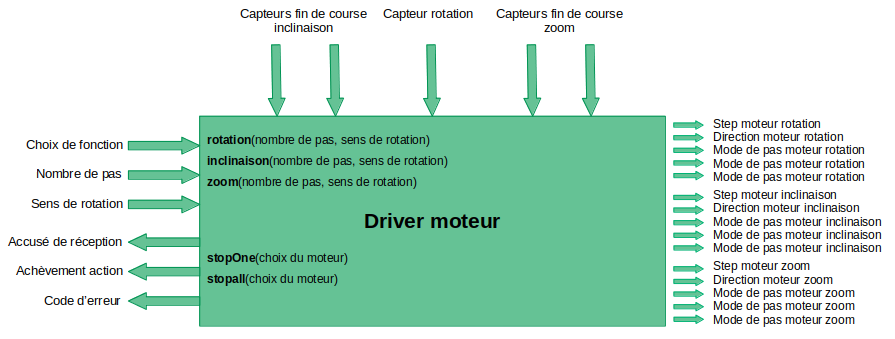
\includegraphics[width=1\linewidth]{\figures/illustration_entree_sortie_driver_moteur.png}
    \decoRule
    \caption[
    Schéma des entrées / sorties du driver moteur]{
    Schéma des entrées / sorties du driver moteur}
    \label{fig:Schéma des entrées / sorties du driver moteur}
    \end{figure}

\vspace{1cm}

La figure 9.1 représente le driver contrôlant les moteurs. À gauche du block il y a les entrées et les sorties du driver d'un point de vue informatique. \newline Les entrées regroupe l'ensemble des données que attent le driver pour entreprendre une action, nous retrouvons de se fait, le choix de l'action à réaliser, le nombre de pas à parcourir, et le sens de rotation et le choix du moteur. Les choix des actions à faire sont en gras à l'intérieur du block Driver. Comme vous pouvez le voire toutes les actions n'ont pas besoin de toutes les informations demander en entrées (comme l'action StopOne), dans ces cas seules les entrées necessaires seront prises en comptes.\newline Concernant les sorties informatiques, il y a l'acquitement de réception qui à pour but de rassurer l'application en lui indiquant se qu'il a reçu, ainsi l'application peut vérifier que les données envoyé sont correctes. Si il y a une erreur de communication l'application demande l'arret des moteurs et renvoi l'ordre ajusté (en prenant en compte le déplacement qui à été effectué dans l'erreur). Nous trouvons ensuite l'achèvement d'action, lorsque une action arrive a son therme (rotation, inclinaison, ...) le driver l'indique à l'application pour quelle que l'ordre est terminé, ainsi si jamais il y a un ajustement à effectuer elle r'enverra un ordre pour bien être placé. Et pour fini se coté informatique, il y a le retour de code d'erreur qu'il survient lorque une incident arrive dans le driver (ressource inaccessible (pin, timer, interrruption), probleme de fermeture driver ou d'ouverture, ...). \newline
Sur le dessus du driver nous trouvons 5 entrées (matérielles) capteurs. Chacun d'eux préviens de l'arrivé en buté d'un axe, hors pour le capteur rotation qui indique juste le position du télescope en rotation lorqu'il est activé. \newline Ce capteur à deux rôles, durant la phase de dévellopement il nous permettra de déterminer le nombre exact et réel du pas pour un tour complet du télescope (se qui permettra de dévelloper l'algorithme de positionnement du télescope dans l'application pricipale). Le second rôle, plus tard, sera de faire du requalibrage de la centrale inertielle en cas de récallage entre entre les résultats ce capteur et la centrale inertielle. \newline
Au final à droite du block nous trouvons les sorties (matérielles) du driver. Ces dernières répètent le même pour chaqu'un des 3 moteurs: une pin pour le front montant pour lancer un pas moteur, le sens de rotation (0 ou 1), et 3 pins pour le choidu mode pas de rotation du moteur (pas complet, demi-pas, ...). \newline
  
 \newline 2 exemples de fonctionnement du driver avec ces entrées/sorties: 
\begin{itemize}
	\item Faire tourner le zoom de 50 pas dans le sens horaire:
	\begin{enumerate}
		\item Reception des nombres de l'application [ 3 ; 50 ; 0 ] pour choisir la fonction zoom, nombre de pas, sens de rotation horaire;
		\item Envoi de l'accusé de réception, à l'application, contenant les nombres 3 ; 50 ; 0 ;
		\item Execution de la fonction zoom avec les données ( 3 50 0 ) en argument.
		\item Ecrit dans la sorte du moteur zoom sens de rotation: 0.
		\item Ecrit en sortie de mode de pas du moteur zoom la configuration pour faire des pas complet. 
		\item Creer un timer qui va permettre de créer un front montant, tant que l'on n'a pas atteint le nombre de pas à parcourir.
		\item Si l'on a parcour tous les pas complet et qu'il faut réaliser des pas plus fins, pour atteindre au plus près l'angle demandé, on change le mode de pas en 16ème de pas. 
		\item Une fois tous les 16ème de pas éffectué on envoi de l'achèvement d'action contenant le nombre 1.
		\item Le driver réinitialise ses variables et ressources (timer,...).
		\item Mise en attente d'un nouvelle ordre, la boucle et bouclé.
	\end{enumerate}
	\item Arreter tout les moteurs
	\begin{enumerate}
		\item Envoi au driver le nombre 5 pour choisir la fonction stopall.
		\item Reception de l'accusé de réception contenant le nombre 5.
		\item Réinitalise les variables et ressources.
		\item Reception de l'achèvement d'action contenant le nombre 1.
	\end{enumerate}
\end{itemize}


Une fois une manoeuvre terminé le driver informe l'application que l'action demandé est arrivé à son terme. Cependant d'un point de vue driver moteur il y a pas de possibilité de vérifier si le télescope est bien placer là où on lui a demander de ce placer. Si une personne ou objet block le mouvement du telescope ou des moteurs ces derniers ne renvairons pas d'avertissement. C'est dont la centrale inertielle qui contrôlera le bon placement du télescope. \newline
Les capteurs de fin de course servent de sécurité, cette partie est indépendante du reste. Elle a pour but d'arrêter un moteur qui à atteint sa position maximale, hormis pour le capteur de rotation qui à pour utilité dans un premier temps de faire une interruption lorsque un tour complet. \newline Avec cette information on pourra déterminer le nombre de pas moteur qu'il faut faire pour faire un tour complet de télescope sur lui même. Et dans un second temps de donner un point de repère pour les recalibrages de la centrale inertielle. \newline 
Les sorties "Mode de pas moteur..." permettent de choisir dans quel mode de rotation doit tourner le moteur (pas complet, demi-pas, quart de pas, huitième de pas, seizième de pas). Augmenter la division de pas permet d’affiner la rotation afin d’atteindre l’angle le plus exact possible à ce qui à été commandé. Ainsi lorsqu'un moteur a accomplie environ 90\% de la distance à réalisé, on change le mode de pas afin d'arriver au plus proche de l'angle exacte.   



\section{Interactions avec le driver}

Le driver est utilisé à partir d'une application situé dans le user-space du linux embarqué. Pour cela j'ai étudié et testées plusieures solutions. \newline
La première qui m'est venu à l'idée était d'utiliser l'IPC (inter process communication). \newline
Une seconde plus archaïque m'est venu à l'idée, celle de partager un ficher entre le programme dans le user-space et du driver. Pour que le programme dans le user-space puisse transférer ses ordres. Cependant je trouve cette solution pas très sécuritaire. \newline
La troisième solution qui m'a été proposé par Vincent Poulailleau est d'utiliser la fonction ioctl. C'est cette solution que j'ai retenu car elle est une technique très rodé dans le domaine car elle était déjà utilisé à la version 7 d'UNIX. 
\vspace{1cm}

\section{Intégration du driver}
Pour que le driver soit utilisable dans le linux embarqué Yocto, j'ai créé deux recettes. L'une viens cherche dans le github du projet le a4988.c (code du driver) et sa librarie (header) header.c , cette recette permet l'importation du driver lors du build du Yocto (avec la commande bitbake). \newline La seconde recette permet d'ajouter l'application d'interface avec le driver dans le user-space du Yocto. Pour lancer l'application dans le Yocto dans la raspberry il suffira d'écrire dans le terminal (de la cible) le nom de l'application: a4988-test \newline 

\section{Validation des fonctionnalitées de bases}

\section{Câblage}
\begin{figure}[H]
    \centering
    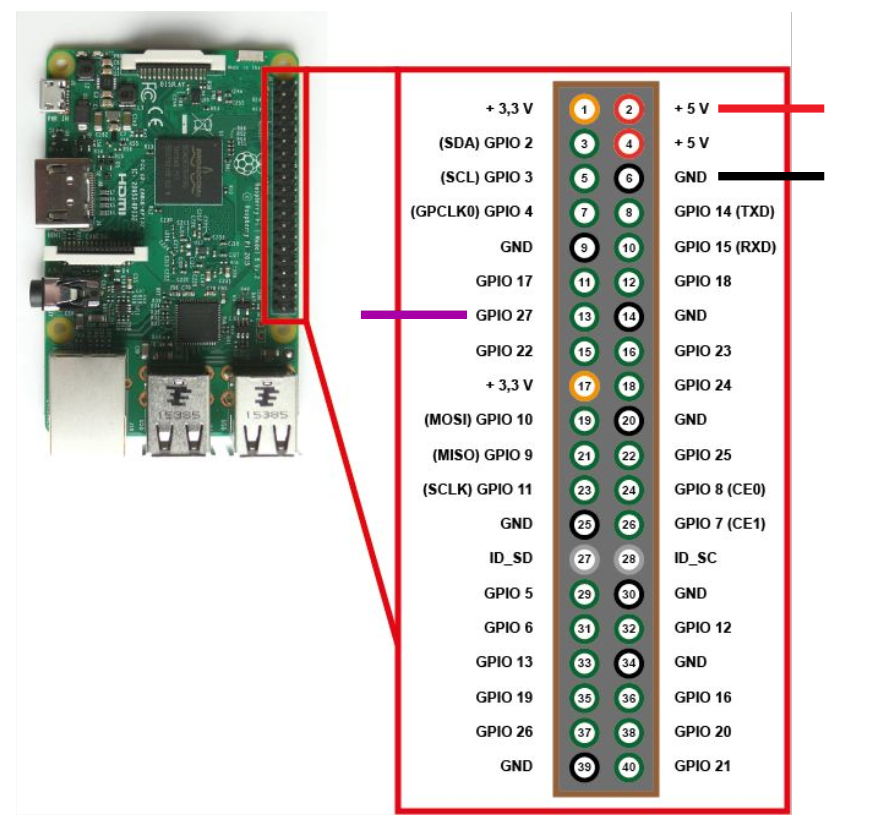
\includegraphics[width=0.5\linewidth]{\figures/sch_pinout.png}
    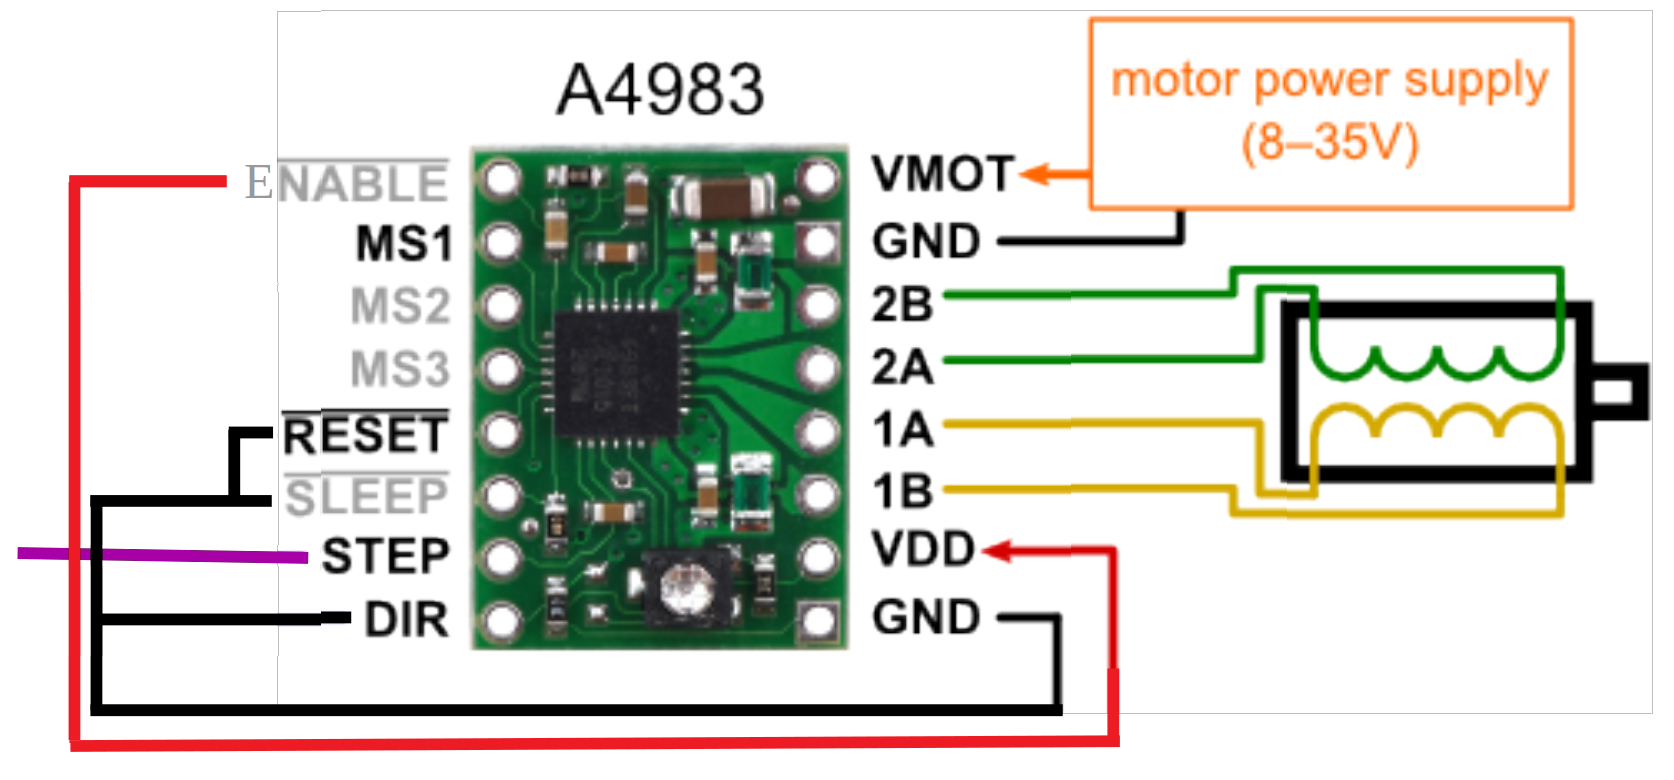
\includegraphics[width=0.5\linewidth]{\figures/sch_a4983.png}
    \decoRule
    \caption[
    Schéma de câblage d'un contrôleur moteur sur la Raspberry Pi]{
    Schéma de câblage d'un contrôleur moteur sur la Raspberry Pi}
    \label{fig:Schéma de câblage d'un contrôleur moteur sur la Raspberry Pi}
    \end{figure}

\vspace{1cm}

Pour valider mon driver, je l’ai testé avec une Raspberry Pi, un contrôleur moteur et un moteur.

\begin{figure}[H]
    \centering
    \includegraphics[width=0.9\linewidth]{\figures/photo_test_motor.jpg}
    \decoRule
    \caption[
    Photo du banc de test]{
	Photo du banc de test}
    \label{fig:Photo du banc de test}
    \end{figure}

\vspace{1cm}

J’ai pu valider les fonctionnalités développées, cependant la vitesse max atteinte par le moteur contrôlé par le driver est inférieure à celle que l'on peut atteindre en contrôlant le moteur avec un générateur basse fréquence.
Voici le résultat de la commande envoyée par la Raspberry Pi par la pin Step au contrôleur moteur pour faire avancer à chaque front montant le moteur de 1 pas.

\begin{figure}[H]
    \centering
    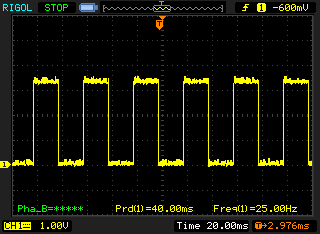
\includegraphics[width=0.5\linewidth]{\figures/osc_motor.png}
    \decoRule
    \caption[
    Mesure à l'oscilloscope de la commande moteur générée]{
	Mesure à l'oscilloscope de la commande moteur générée}
    \label{fig:Mesure à l'oscilloscope de la commande moteur générée}
    \end{figure}

\vspace{1cm}

Après avoir étudié les résultats avec d'autres professeurs, j'ai conclu que la période minimale que je puisse atteindre soit de $20ms$ est normal. Cette limitation est due au fait que mon driver n'a pas la priorité des ressources dans le Linux. Et que le Linux a un cycle lecture/écriture des entrées/sorties limité. Pour améliorer cela il faudrait passer sur un Linux temps réel.


